% !TEX root = thesis.tex
This chapters purpose is to give context to the AES algorithm. It starts with a brief history of cryptography, explains the AES-selection-process and then gives some examples of security issues that have been found over the years.


\section{Before AES}
\label{ch:before-aes}
Cryptography or the art of concealing meaning in writing ist over 4000 years old.

The advent of the electronic computer changed the field of cryptography fundamentally. Starting with the "bombe", produced by Alan Turing and refined by Gordon Welchman around 1940, the world ushered into a new era of automated de- and encryption. 
The bombe is an electro-mechanical device that was key to breaking the ciphers produced by the enigma - a device used by the german military in the second world war to secure their communications. Turings bombe was the first machine that was able to break message encryption in an automated fashion. Previously cryptoanalysts had to break ciphers "by hand" i.e. by doing manual frequency analysis for example. Breaking the enemies communication provided a vital advantage for the Allies during World War Two.
The next cryptographic revolution came in 1971 when Whitfield Diffie invented public-key-cryptography, single-handedly eliminating a problem that haunted cryptographers from the beginnigs of their field of expertise: the establishing of a shared secret over insecure channels, also known as the key distribution problem. Previously the security of an encryption scheme based on the fact, that there was atleast one element in said scheme, that must remain unknown to malicious parties intending to attack and decipher the communication, for example a password. Public-key-cryptography does not work like this: Parties wishing to communicate simply exchange their public keys over an unsecured channel and are able to establish a guaranteed shared secret from that. Without knowing the corresponding private keys, the public keys are worthless in the eyes of an attacker. But the maths behind Public-key-cryptography is prohibitively expensive if one attemts to encrypt something this way by hand. Progress like this was only possible by utilising electronic computers.
When those computers later on became widely available for a broader range of people, suddenly everyone was able to encrypt information with complicated schemes. And for the first time the security of those schemes was mathematically provable. In fact the prove of some of those later schemes guaranteed protection even from entities with massive resources, manpower and expertise without the need for skilled and qualified cryptographers. 
The first openly available standart for electronic encryption was a symmetric cipher called "Data Encryption Standard" or DES. Developed in the early 1970s at IBM the cipher was published in 1977 as an official Federeal Information Processing Standard (FIPS). The security of DES was disputed right from its first publication. Even in the late seventies the key length was critisized as too short, although it took until June of 1997 before the first DES message was publicly decrypted via brute force attack. In January of the same year the search for a predecessor of DES was announced by the National Institute of Standards and Technology of the United States (NIST). This predecessor supposed to be "an unclassified, publicly disclosed encryption algorithm capable of protecting sensitive government information well into the next century." To increase trust into this standard-to-be the search was public and NIST relied on submissions from the cryptographic community. 


\section{The Advanced Encryption Standart selection}
\label{ch:aes-selection}

The following chapter is, if not mentioned otherwise, based on \cite{nistdevoverview}.

The formal call for submissions of AES canidates came in september of 1997. NIST explicitly requested input from outside of the institution by explicitly asking "the public, academic/research communities, manufacturers, voluntary standards organizations, and Federal, state, and local government organizations." The submissions would be made public for review and comment after the submission period

\subsection{Requirements}
\label{ch:requirements}

The proposed algorithms for the new encrytion standard and thus the
potential successors of DES had to fullfill a number of requirements, as can be found in \cite{announcementrequest}, in order for them to be concidered by NIST. AES was intended to be a block
cipher operating on 128 bits at a time. Those bits should be secured by
key length of atleast the three sizes 128, 192 and 256 bits. 
The canidates would be furthermore analyzed and evaluated regarding:

\begin{itemize}
\item
  \emph{security}: Deemed as the most important criterion, it
  encompasses factors like the actual security compared to the
  competitors, the degree to which the algorithm is able to produce an
  output indistinguishable to a random permutation of the input, the
  quality of the mathematical prinicples behind the algorithm and of
  course critique, concerns and attacks regarding the canidate
  originating from the public review.
\item
  \emph{cost}: Financial cost was one concideration: All canidates had
  to be released on a ``worldwide, non-exclusive, royalty-free basis.''
  before they could be submitted. Performance costs like the speed of
  the algorithm both in software and hardware implementations or memory
  size, be it in code size, gate count for hardware implementations or
  RAM requirements for software implementations were further factors
  that played a role in this category.
\item
  \emph{algorithm and implementation characteristics}: Flexibility
  without compromising security was another desirable aspect of the new
  standard. Additonal key sizes to those specified in the minimum
  requirements, the possibility of implementation on a variety of
  platforms, from slower 8-bit SmartCard processors to fully-fledged
  desktop CPUs and other fields of applications like usage as a stream
  cipher, message authentication generator, pseudorandom number
  generator, hashing algorithm and more were all attributes to the
  flexibility of an encryption algorithm an thus factors, that
  influenced the AES-comittee in their final decision. The last aspect
  under which the standard-to-be had to prove itself was simplicity,
  where a simpler algorithm, that holds up well under all other aspects,
  is preferable.
\end{itemize}


\subsection{The AES selection process}
\label{ch:aes}


Nearly a year after requesting submissions, NIST published a list with fifteen canidates they deemed worthy of further investigation at the First AES Canidate Conference (AES1) in August 1998. The cryptographic community was invited to critique those choices, either via email or later on in the online discussion forum NIST hosted for this exact purpose. This input from the community collected in "Round 1" of the selection process was discussed at the Second AES Canidate Conference (AES2) in spring of 1999. Shortly after that NIST selected in their publication \cite{round1report} five finalists from the initial fifteen algorithms: MARS, RC6, Rijndael, Serpent, and Twofish.
The other canidates were excluded, partially because "serious questions [had] been raised about [their] security" (p.34), partially because they were slower/potentially less secure than other comparable canidates.
The finalists moved on to recieve further scrutiny from both the NIST and the cryptographic community in the so called "Round 2".
After this more in-depth analysis of the algorithms a third conference (AES2) in April 2000 provided an open, public forum to review and discuss the findings accumulated up to this point in Round 2. The authors of the finalists were explicitly invited to partake in the process. A month later Round 2 came to an end and NIST moved on to select the algorithm they deemed to be best suited to be the Advanced Encryption Standard. 
On October of the same year the institute announced in \cite{round2report} their decision to propose Rijndael, authored by Joan Daemen and Vincent Rijmen, as the AES. Each finalist "appears  to  offer adequate security, and each offers a considerable number of advantages" (p.91), but "Rijndael’s combination of security, performance, efficiency, implementability, and flexibility make it an appropriate selection for the AES" (p.92).
The proposal was formalized in a FIPS draft for AES and published on February 2001 (\cite{fipsdraft}. After going throught the usual FIPS-approval-process the Advanced Encryption Standard was made public as FIPS 197 \cite{fips197} at the end of the year.

\begin{figure}
\centering
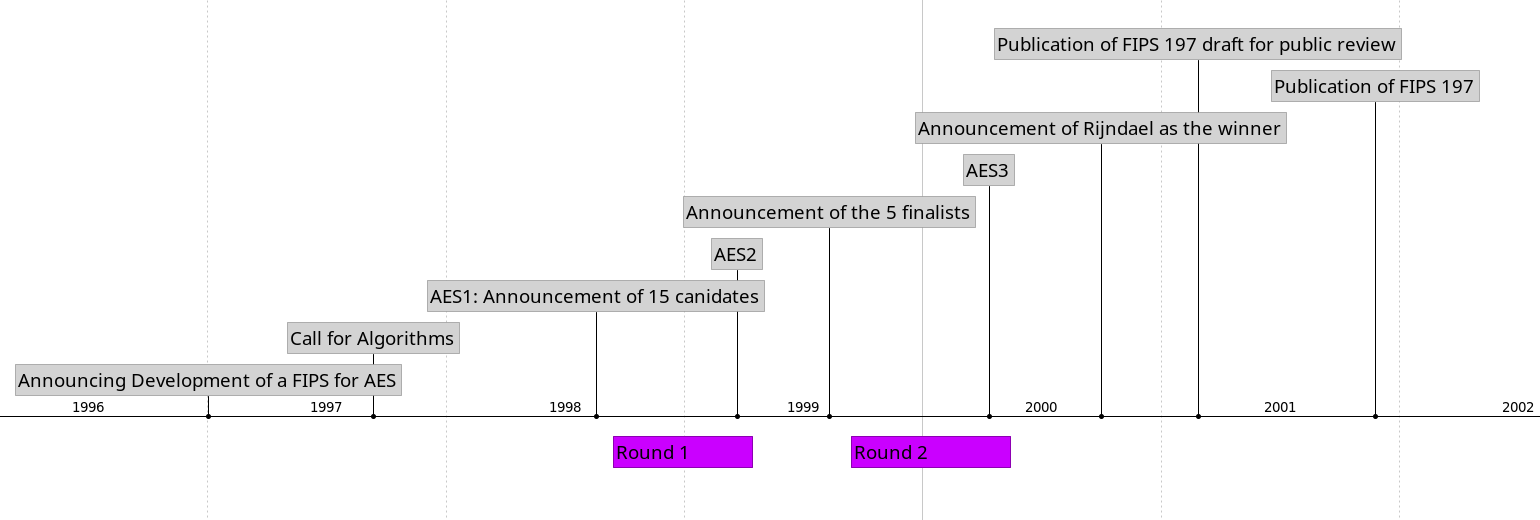
\includegraphics[scale=0.35]{aes-process-timeline.png}
\caption{AES selection process timeline}
\end{figure}

\section{AES in review}
\label{ch:aes-review}

The slightly modified Rijndael that is known as AES today has been subject to a lot of analysis over the years, with many focussing on the security aspects of the algorithm.

\subsection{NIST}
\label{ch:nist-review}

From their Round-2-Report \cite{round2report} can gain some insight in how NIST thought about Rijndael in detail. 
Although they acknowledged that some voiced critisism regarding its mathematical structure offering a potential attack vector on the algorithm, they believe that the simplicity of said structure facilitated a deeper understanding of the security properties Rijndael brings to the table. Overall they report to have no knowledge of a security attack against Rijndael.
Performance-wise they emphasise the good performance of the algorithm under a variety of circumstances, be it 8- or 64-bit software implementations, the ease, with which the algorithm is able to run in an parallel setup, the fast key setup time, low memory and disk space footprints and the speed of the hardware implementation.
NIST states that Rijndael is -thanks to its operations used- one of the easiest algorithms of the finalist to defend against power and timing sidechannel attacks. The institute did not notice a great hit in performance while testing a hardened version of Rijndael, atleast in comparison to the other finalists. Some power analysis attacks still seem to be effective though, even with the hardended Rijndael.
Key setup time and key agility were two other strong areas for Rijndael in the eyes of NIST. Furthermore the authors hint at the possibility of flexible key and block sizes, which, while not really concidered at the time of the report, is another sign in favor of Rijndael.

\subsection{Side Channel Attacks}
\label{ch:sidechannelattacks}

The cryptographer Bernstein described in \cite{bernsteincache} a successful key-extraction via network from the OpenSSL AES implementation running on a Pentium III (both very common software and hardware at the time). This sidechannel attack was in his eyes not a result of a faulty implementation, but an inherent flaw in the design of the algorithm that makes it "extremely difficult to write constant-time high-speed AES software for common general-purpose CPUs." (p.1). In many cases Bernstein can make out a correlation between the time it takes to load an array entry and the index of an entry in said array. Thus the time it takes to load an entry leaks information about the information currently processed within the algorithm ultimately revealing the key to an attacker, if said attacker can piece the leaked information together in the right way.
According to Bernstein, this is not only a problem inherent to AES, but to all cryptographic algorithm implementations that rely heavily on lookup tables to speed up their computation.
\cite{improvedcache} XXX states, that while Bernsteins "approach is widely applicable" (p.205) it critizizes this approach, because one requirement is the collection of timing data from approcimately \[2^{27.5}\] encrypted samples. Furthermore the fragility of the Bernsteins attack is one of the main drawbacks according to te authors. The attacker needs to replicate the targeted machine with a lot of care, since small differences between target and replication will produce unusable timing data, leading to failure of the attack. Their own cache-collision timing attacks -while being orders of magnitude faster under optimal circumstances than the previously discussed attack- are representing "a significant step towards developing realistic remote timing attacks against AES" (p.210).
The power draw of the encrypting CPU seems to represent another attack vector on the algorithm. In \cite{powerdraw} the authors force the eviction of selected parts of AES lookuptables (like the SBOX) and measure the increased power draw from the CPU in case of a cache miss in the following encryption calculations. With that the authors claim to be able to extract the complete secret key. While the attack itself is descibed as "quite simple" (p.6), the same statement is made for the proposed countermeasure.
\cite{ctattacksfeasible} finds that the ease of AES-cache-behaviour exploitation is not neccessarily true anymore on more modern x86-processors. Features like multiple cores per processor with each having its own cache, the increased cache pressure emmited from more complex software, physically tagged caches, the partially undocumented and very complex prefetcher units and of course the AES-NI instruction set make it "substantially more difficult to mount data-cache side-channel attacks on AES than previously realized." (p.1). As in \cite{aes-ni} stated, AES-NI itself promises to prevent some software sidechannel attacks singlehandedly by sheer virtue of not having to use lookuptables for a fast implementation of the encryption algorithm.
This does not neccessarily apply to the slew of novel attacks categorized as 'transient execution CPU vulnerabilities' (see \cite{transientexecution}), but since they do not target AES directly they will not be discussed here.

\subsection{Mathematical Attacks}
\label{ch:mathematicalattacks}

During the AES developement the first papers with attacks on Rijndael were published. \cite{Gilbert00acollision} demonstrated an attack that broke seven rounds of AES with any key length, but the attacks "complexity is very high even if the number of plaintexts to cipher is small." (p.11). The authors did not see a danger to the complete 10-round-version.
Roughly around the same time \cite{impcryptan} published and attack, that managed to break one round more for each AES-192 and AES-256, but "[m]any of these attacks require virtually the entire codebook of texts and hence are not very practical." (p.15).
The key schedule of Rijndael was critisized in the same paper, the authors found it "worrisome" (p.15). \cite{rkeyattack} expressed similar concerns, even going as far as labeling it as weak, since it was for example enabling related-key attacks on the full rounds of AES-192 and AES-256 algorithm, which the authors found out earlier in \cite{rkeyattack2}.  While those attacks "are still mainly of theoretical interest [at the time] and do not present a threat to practical applications using AES" (p.14), or related-key attacks in general are not " not universally accepted as a practical attack model."\cite{rkeyattack3} (p.14) they also "should not be possible in a good cipher." \cite{rkeyattack} (p.13). 
\cite{rkeyattack3} continues chipping away at the confidence held in the 256-bit variant of AES, describing key derivation attacks "of practical complexity" (p.2) on a 10-round variant of that algorithm. The authors identify again the design of the key-schedule as a culprit, which they deem "not of industrial strength" (p.14). The attack seems ineffective against the 128-bit variant of the encryption algorithm. Nevertheless the authors are of the opinion, that "AES can no longer be considered as a safe black box construction, which can be dropped into any security application with little thought about how it is used."(p.14), a notion, which they think of as "disturbing"(p.14).
One of the most successful attacks on the algorithm was described in \cite{biclique} where the authors used Biclique Cryptanalysis to mount a better-than-brute-force-attack on AES with all rounds used as described in the standard, effecively reducing the key strength of each AES variant by a few bits. But even with this novel approach it still remains infeasible to recover a AES-encrypted plaintext from a ciphertext without the key or usage of side channels.
